\color{black}
{\color{secblue}\subsection{External interface requirements}}
{\color{secblue}\subsubsection{User Interfaces}}

The following mockups offer an intuitive view of what the final product will look like.

\begin{figure}[H]
\centering
\begin{subfigure}{.33\textwidth}
  \centering
  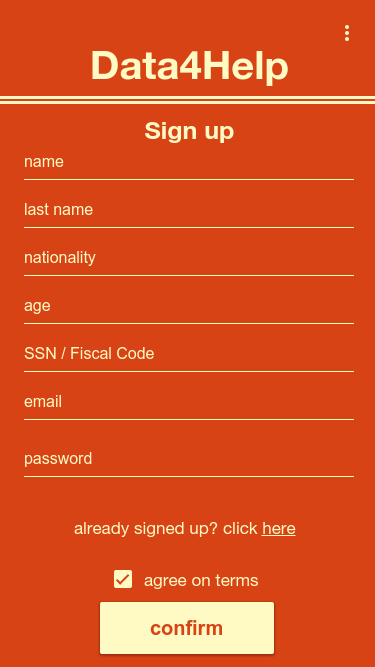
\includegraphics[width=.9\linewidth, height = 7cm, keepaspectratio]{./Images/Mockups/Data4Help/D4HU/D4HU_SignUp.png}
  \caption{Data4Help - User - Sign Up}
\end{subfigure}%
\begin{subfigure}{.33\textwidth}
  \centering
  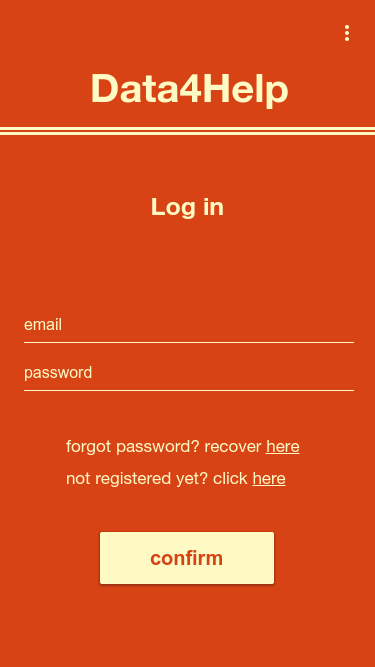
\includegraphics[width = .9\linewidth, height = 7cm, keepaspectratio]{./Images/Mockups/Data4Help/D4HU/D4HU_Login.png}
  \caption{Data4Help - User - Login}
\end{subfigure}
\begin{subfigure}{.33\textwidth}
  \centering
  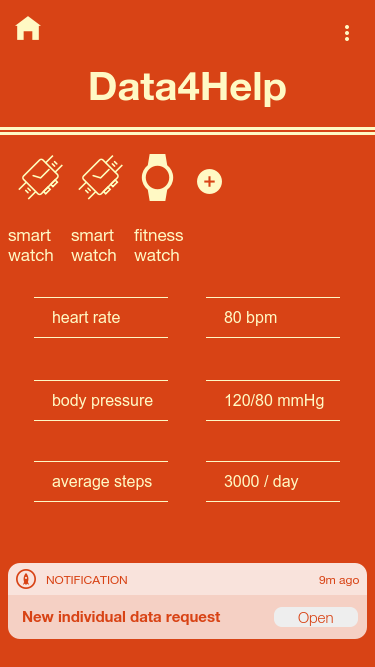
\includegraphics[width = .9\linewidth, height = 7cm, keepaspectratio]{./Images/Mockups/Data4Help/D4HU/D4HU_Homepage.png}
  \caption{Data4Help - User - Homepage}
\end{subfigure}
\end{figure}


\begin{figure}[H]
\centering
\begin{subfigure}{.5\textwidth}
  \centering
  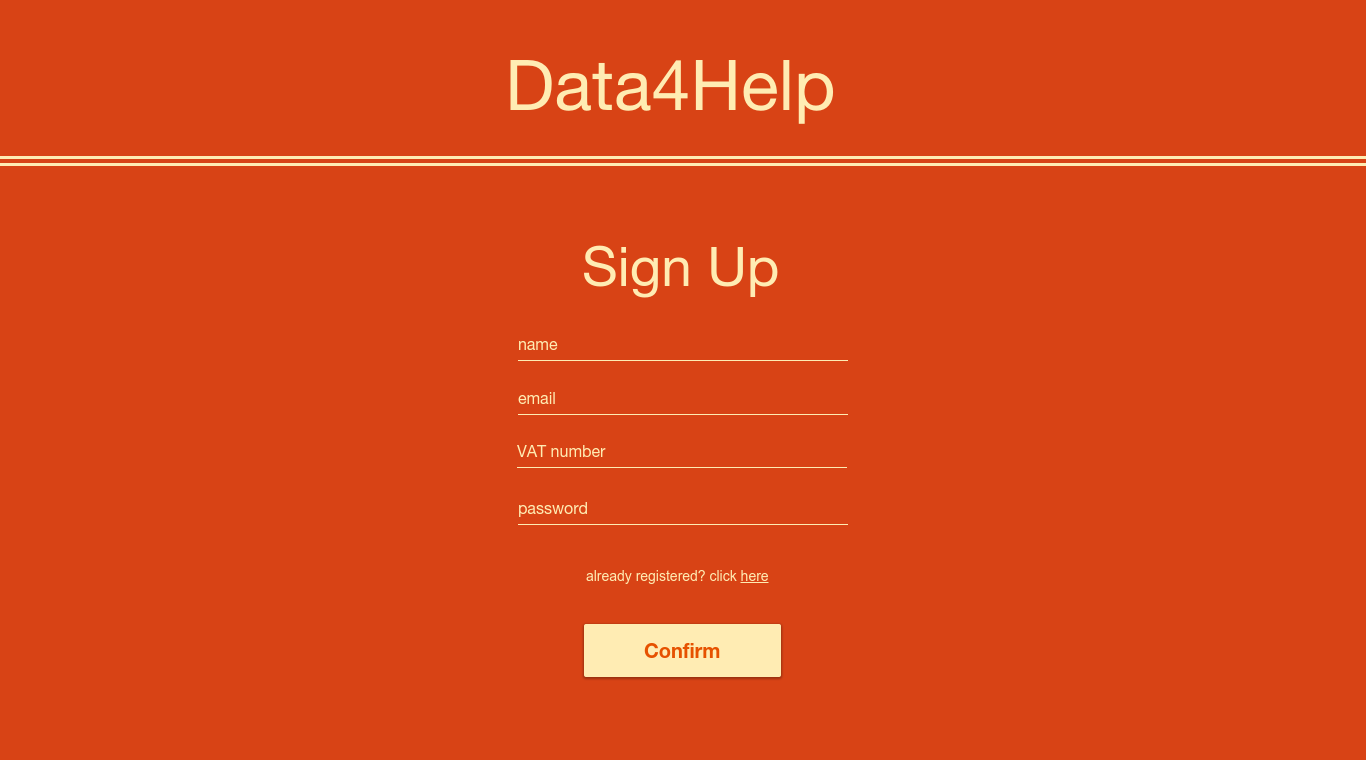
\includegraphics[width=.9\linewidth, height = 7cm, keepaspectratio]{./Images/Mockups/Data4Help/D4HTP/D4HTP_SignUp.png}
  \caption{Data4Help - Third Party - Sign Up}
\end{subfigure}%
\begin{subfigure}{.5\textwidth}
  \centering
  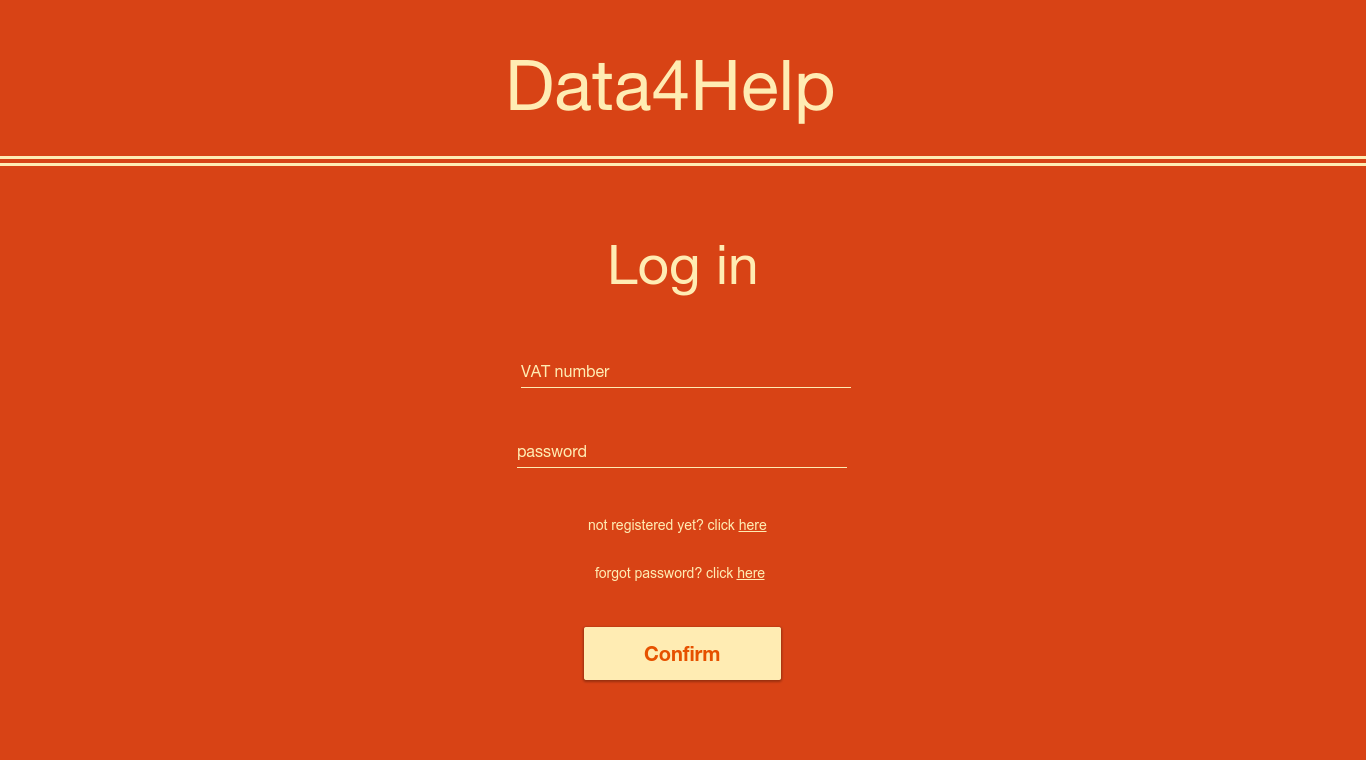
\includegraphics[width = .9\linewidth, height = 7cm, keepaspectratio]{./Images/Mockups/Data4Help/D4HTP/D4HTP_Login.png}
  \caption{Data4Help - Third Party - Login}
\end{subfigure}
\end{figure}

\paragraph{D4HTP - Homepage}
\begin{figure}[H]
    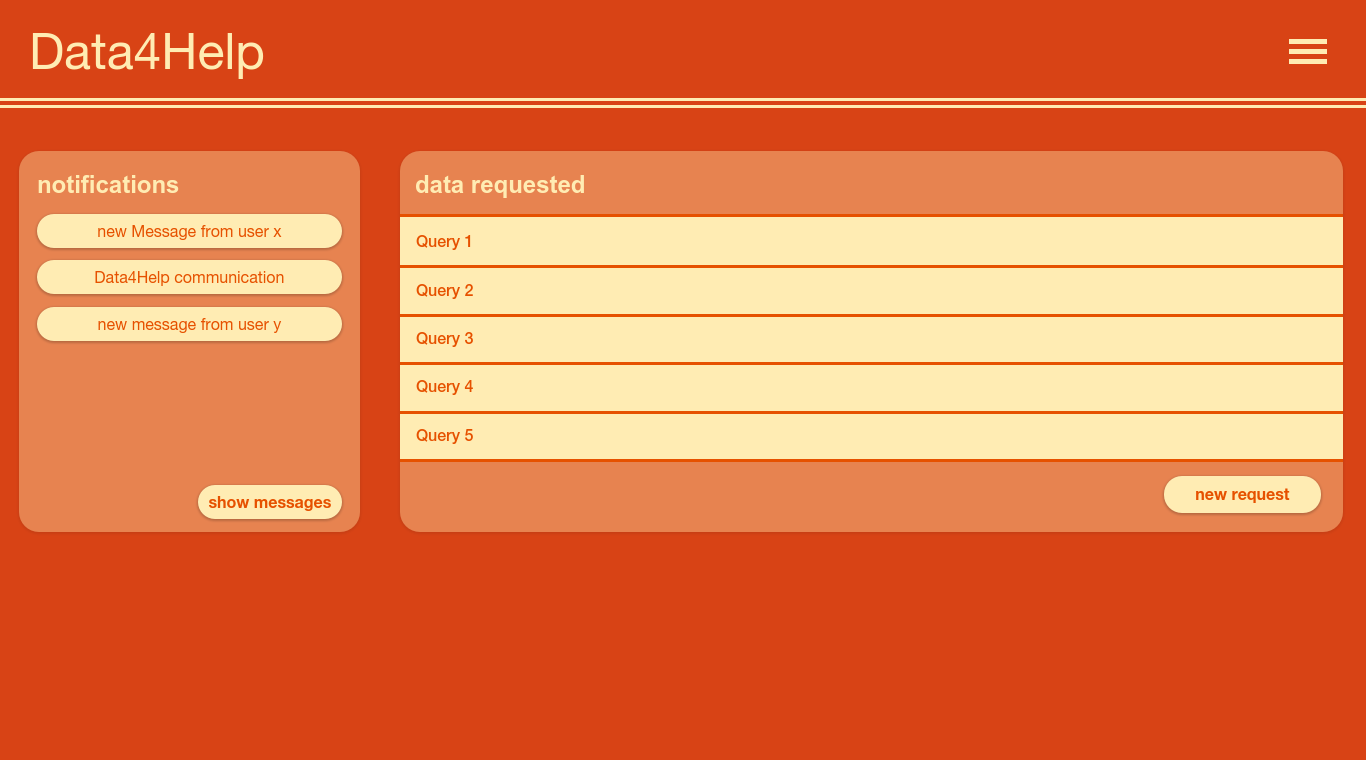
\includegraphics[width=.6\linewidth, height = 20cm, keepaspectratio]{./Images/Mockups/Data4Help/D4HTP/D4HTP_HomePage.png}
    \centering
    \caption{Data4Help - Third Party - Homepage}
    \label{fig:sab}
  \end{figure}

\begin{figure}[H]
    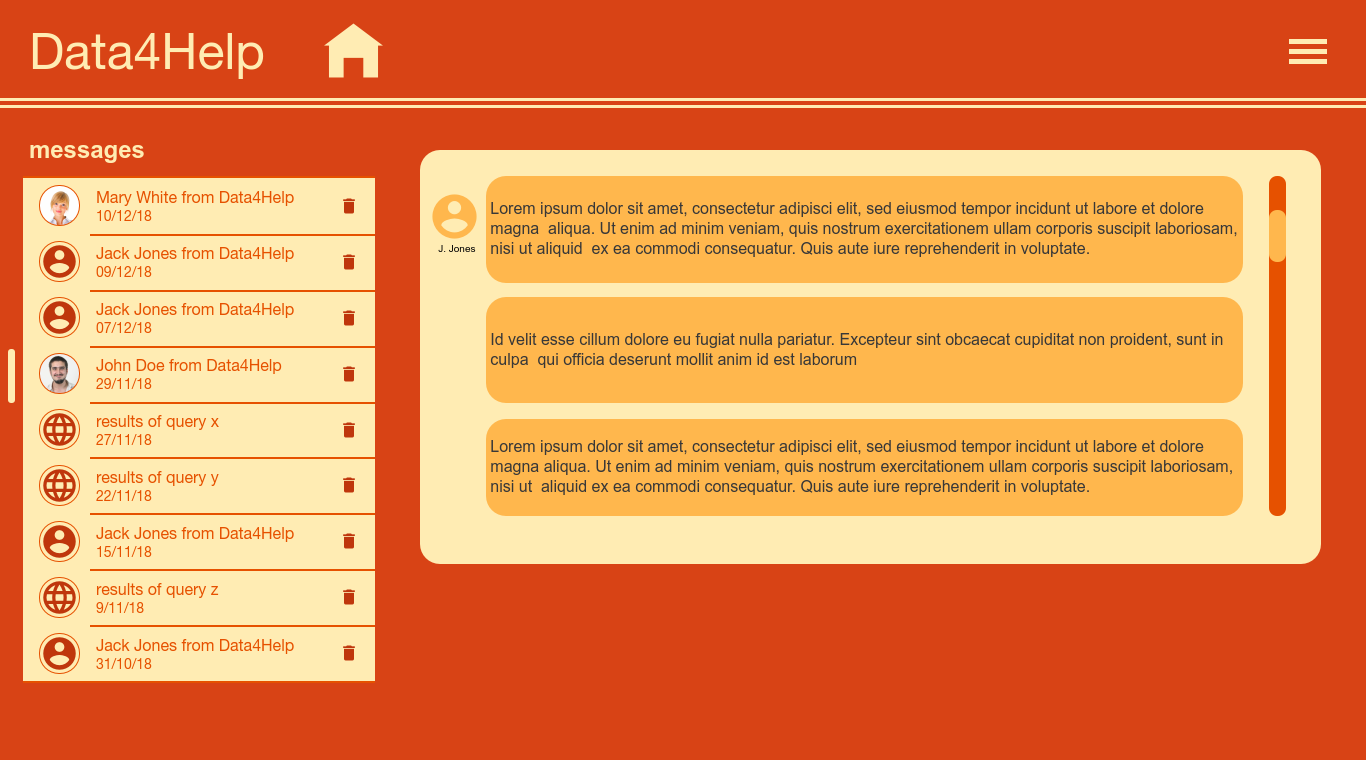
\includegraphics[width=.6\linewidth, height = 20cm, keepaspectratio]{./Images/Mockups/Data4Help/D4HTP/D4HTP_ShowMessages.png}
    \centering
    \caption{Data4Help - Third Party - Messages}
    \label{fig:sab}
\end{figure}


\begin{figure}[H]
    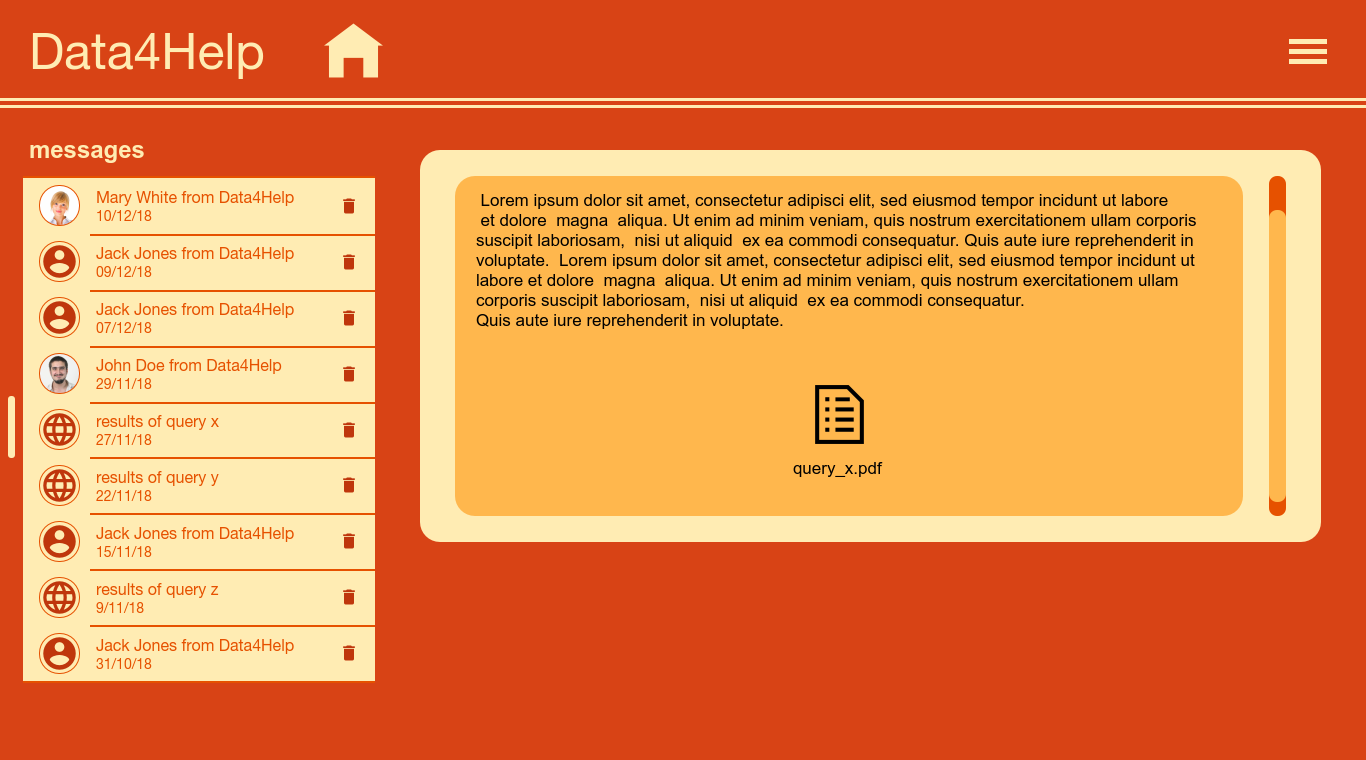
\includegraphics[width=.6\linewidth, height = 20cm, keepaspectratio]{./Images/Mockups/Data4Help/D4HTP/D4HTP_ShowQuery.png}
    \centering
    \caption{Data4Help - Third Party - Messages - Query Result}
    \label{fig:sab}
  \end{figure}


\begin{figure}[H]
    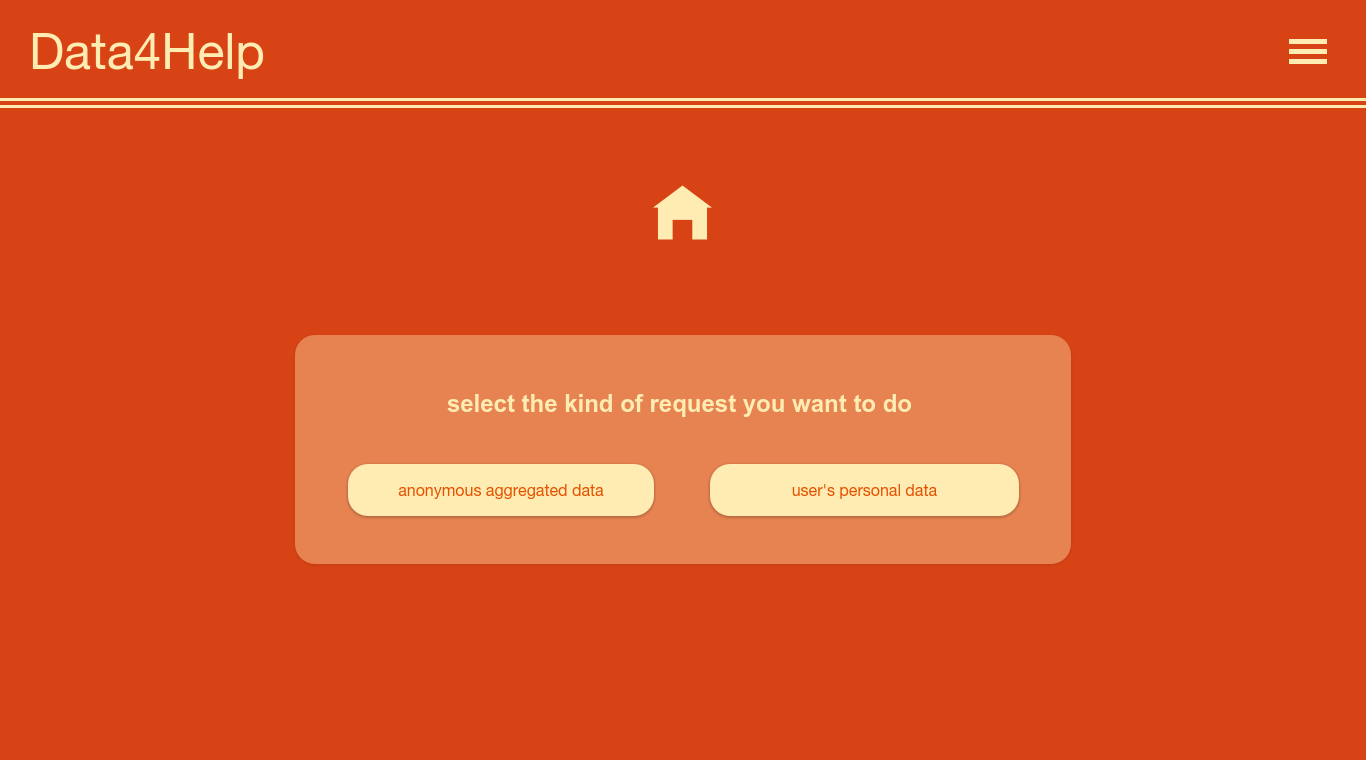
\includegraphics[width=.6\linewidth, height = 20cm, keepaspectratio]{./Images/Mockups/Data4Help/D4HTP/D4HTP_NewQueryRequest.png}
    \centering
    \caption{Data4Help - Third Party - New Query Request}
    \label{fig:sab}
\end{figure}


\begin{figure}[H]
  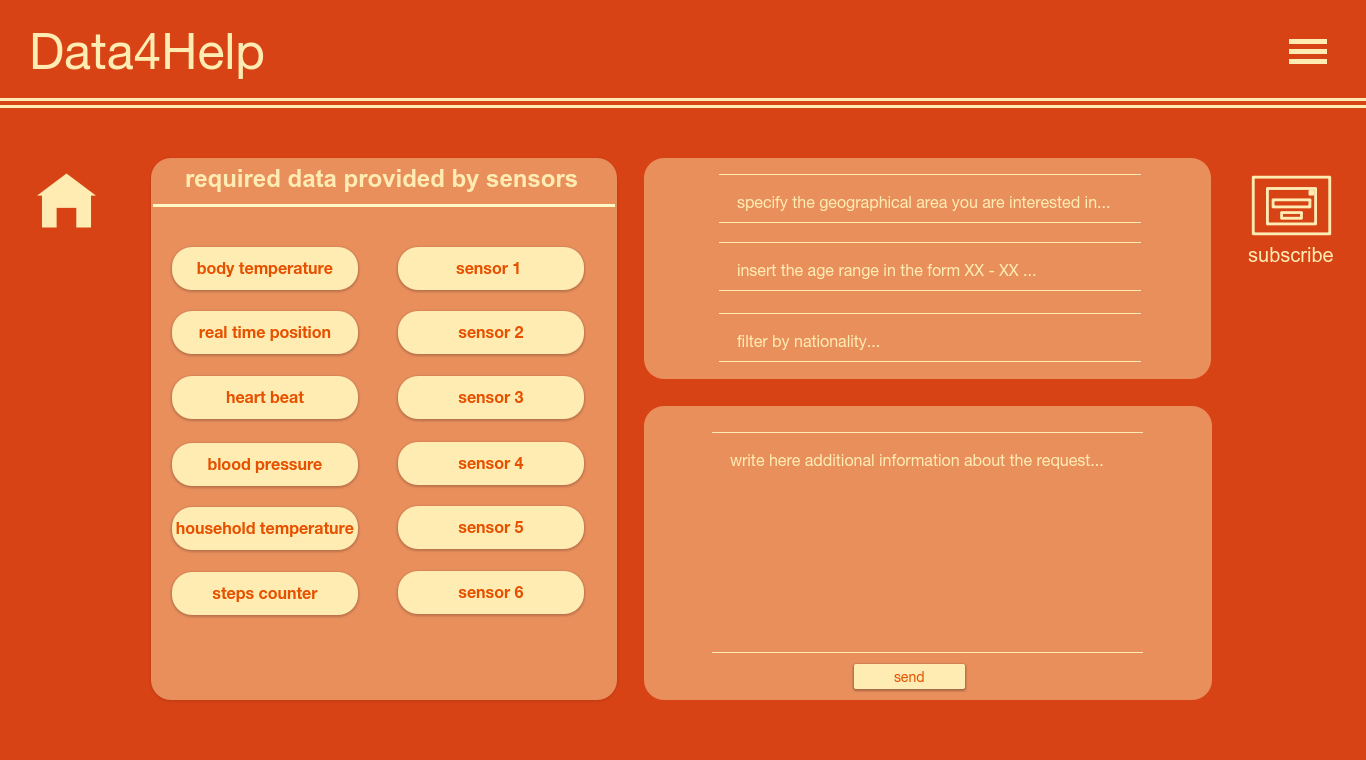
\includegraphics[width=.6\linewidth, height = 20cm, keepaspectratio]{./Images/Mockups/Data4Help/D4HTP/D4HTP_AggregatedDataRequest.png}
  \centering
  \caption{Data4Help - Third Party - Aggregated Data Request}
  \label{fig:sab}
\end{figure}

\begin{figure}[H]
    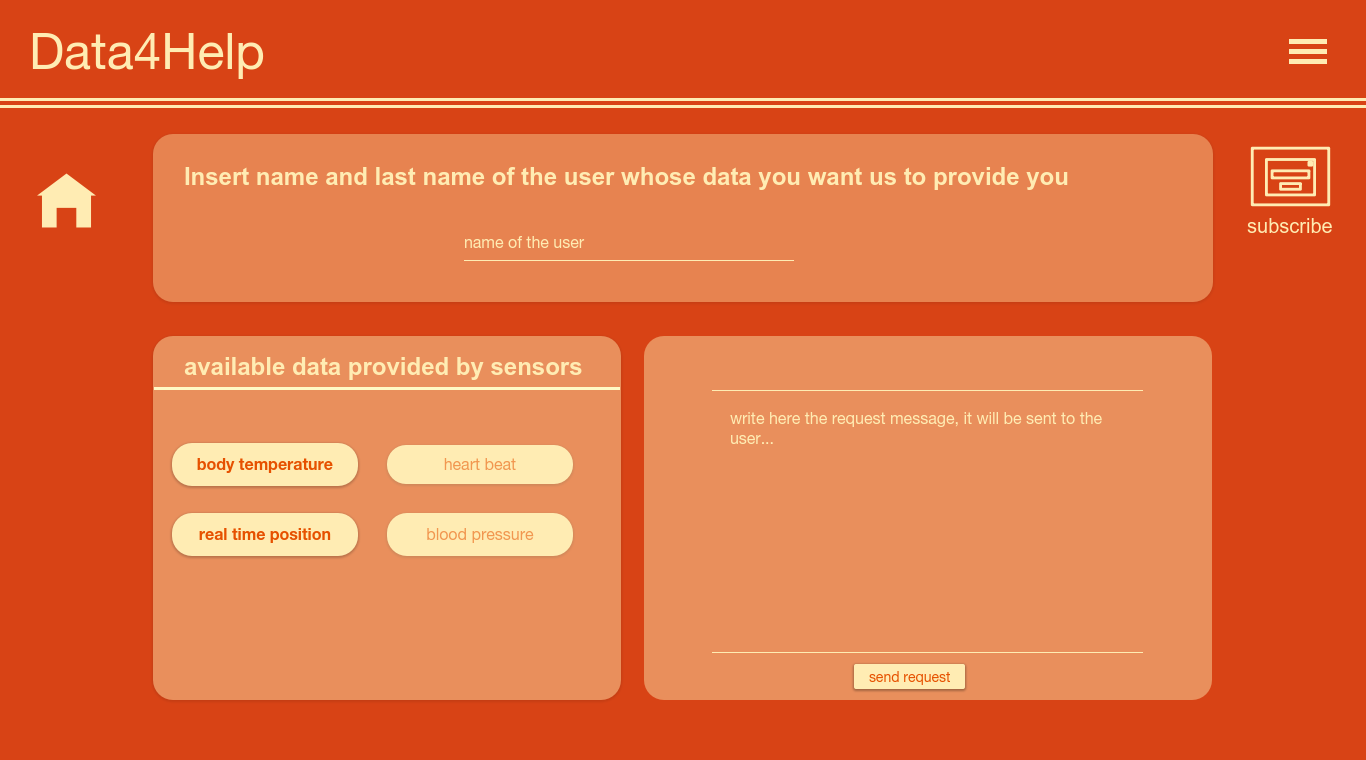
\includegraphics[width=.6\linewidth, height = 20cm, keepaspectratio]{./Images/Mockups/Data4Help/D4HTP/D4HTP_IndividualDataRequest.png}
    \centering
    \caption{Data4Help - Third Party - Individual Data Request}
    \label{fig:sab}
 \end{figure}


\begin{figure}[H]
\centering
\begin{subfigure}{.33\textwidth}
  \centering
  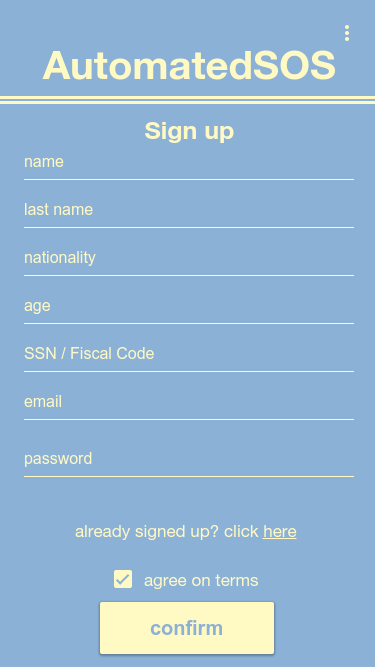
\includegraphics[width=.9\linewidth, height = 7cm, keepaspectratio]{./Images/Mockups/AutomatedSOS/ASOS_SignUp.png}
  \caption{AutomatedSOS - Sign Up}
\end{subfigure}%
\begin{subfigure}{.33\textwidth}
  \centering
  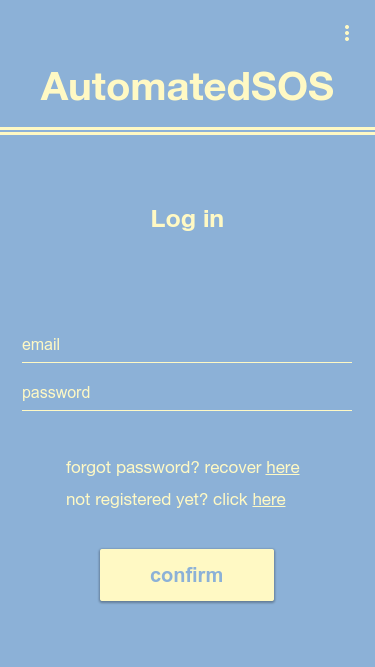
\includegraphics[width = .9\linewidth, height = 7cm, keepaspectratio]{./Images/Mockups/AutomatedSOS/ASOS_Login.png}
  \caption{AutomatedSOS - Login}
\end{subfigure}
\begin{subfigure}{.33\textwidth}
  \centering
  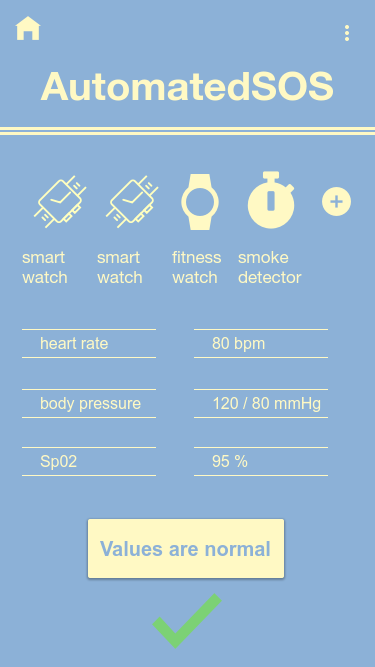
\includegraphics[width = .9\linewidth, height = 7cm, keepaspectratio]{./Images/Mockups/AutomatedSOS/ASOS_Homepage.png}
  \caption{AutomatedSOS - Homepage}
\end{subfigure}
\end{figure}


\begin{figure}[H]
\centering
\begin{subfigure}{.33\textwidth}
  \centering
  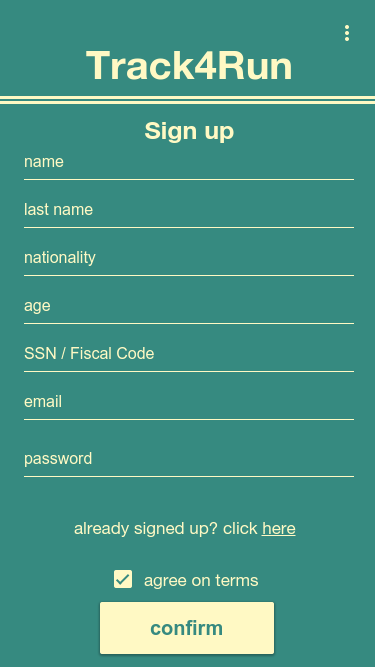
\includegraphics[width=.9\linewidth, height = 6.8cm, keepaspectratio]{./Images/Mockups/Track4Run/T4R_SignUp.png}
  \caption{Track4Run - Sign Up}
\end{subfigure}%
\begin{subfigure}{.33\textwidth}
  \centering
  \includegraphics[width = .9\linewidth, height = 6.8cm, keepaspectratio]{./Images/Mockups/Track4Run/T4R_Login.png}
  \caption{Track4Run - Login}
\end{subfigure}
\begin{subfigure}{.33\textwidth}
  \centering
  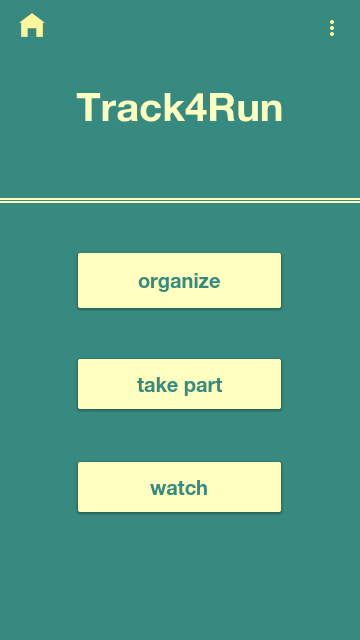
\includegraphics[width = .9\linewidth, height = 6.8cm, keepaspectratio]{./Images/Mockups/Track4Run/T4R_Homepage.png}
  \caption{Track4Run - Homepage}
\end{subfigure}
\end{figure}

\begin{figure}[H]
\centering
\begin{subfigure}{.5\textwidth}
\centering
    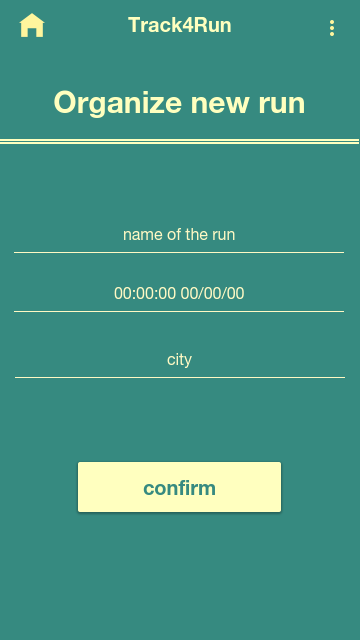
\includegraphics[width=.9\linewidth, height = 6.8cm, keepaspectratio]{./Images/Mockups/Track4Run/T4R_Organize.png}    
    \caption{Track4Run - Organize}
  \end{subfigure}%
\begin{subfigure}{.5\textwidth}
\centering
    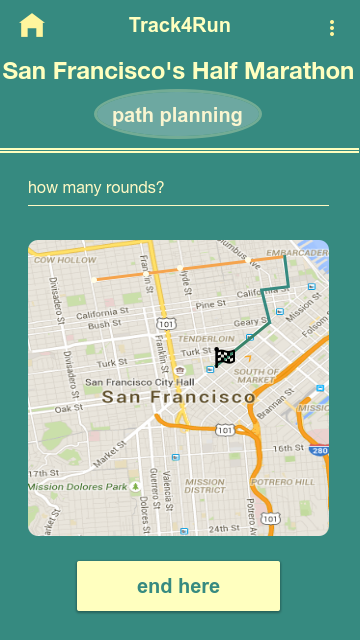
\includegraphics[width=.9\linewidth, height = 6.8cm, keepaspectratio]{./Images/Mockups/Track4Run/T4R_Organize_SetPath.png}
    \caption{Track4Run - Organize - Set Path}
  \end{subfigure}
\end{figure}



\begin{figure}[H]
\centering
\begin{subfigure}{.5\textwidth}
    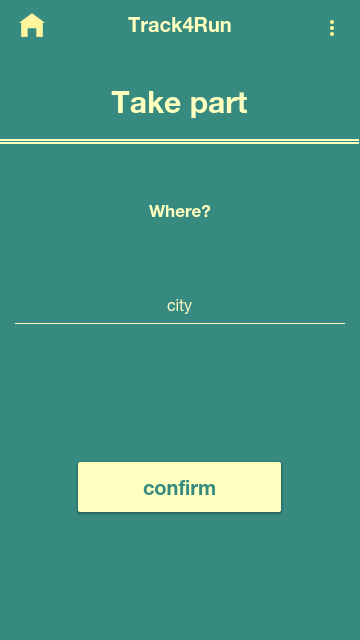
\includegraphics[width=.9\linewidth, height = 6.8cm, keepaspectratio]{./Images/Mockups/Track4Run/T4R_TakePart1.png}
    \centering
    \caption{Track4Run - Take Part - Step 1}
  \end{subfigure}%
\begin{subfigure}{.5\textwidth}
    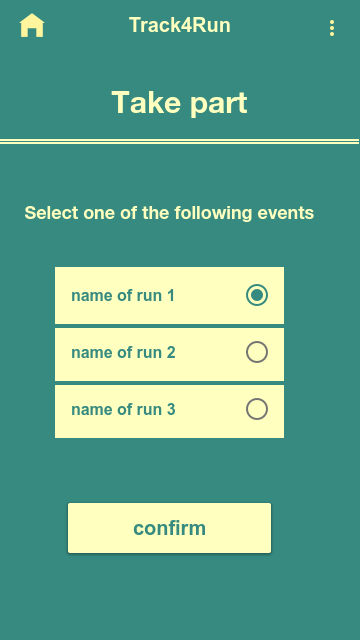
\includegraphics[width=.9\linewidth, height = 6.8cm, keepaspectratio]{./Images/Mockups/Track4Run/T4R_TakePart2.png}
    \centering
    \caption{Track4Run - Take Part - Step 2}
  \end{subfigure}
\end{figure}
  



\begin{figure}[H]
\centering
\begin{subfigure}{.5\textwidth}
    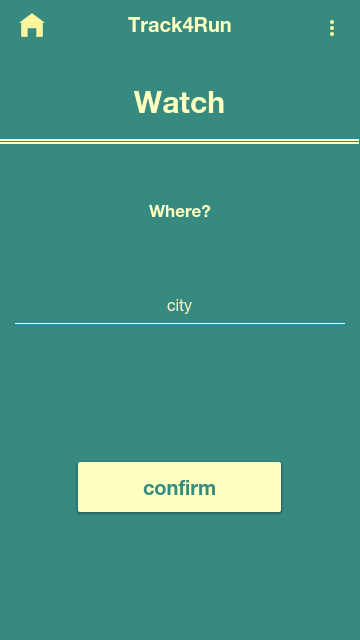
\includegraphics[width=.9\linewidth, height = 6.8cm, keepaspectratio]{./Images/Mockups/Track4Run/T4R_Watch.png}
    \centering
    \caption{Track4Run - Watch}
  \end{subfigure}%
\begin{subfigure}{.5\textwidth}
    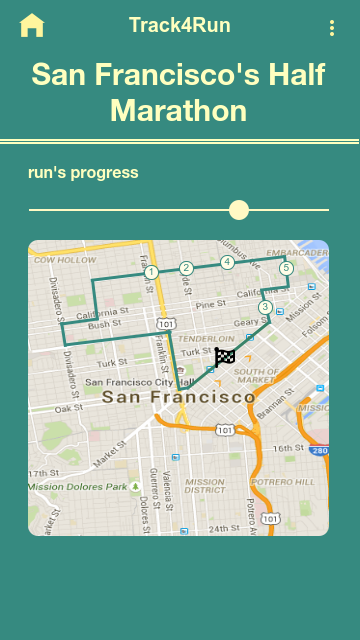
\includegraphics[width=.9\linewidth, height = 6.8cm, keepaspectratio]{./Images/Mockups/Track4Run/T4R_Watch_Map.png}
    \centering
    \caption{Track4Run - Watch - Map}
  \end{subfigure}
\end{figure}


{\color{secblue}\subsubsection{Hardware Interfaces}}
[R1] - This application needs a data warehouse to store all the user data and to allow high performance researchs with large amount of data. This is done using the Amazon AWS services.
{\color{secblue}\subsubsection{Software Interfaces}}
\begin{itemize}
\item{} [R2] - Amazon Redshift as a datawarehouse on top of Amazon S3 to store all the data in an efficent manner;
\item{} [R3] - Google Maps for converting stored GPS data into human readable data for the third parties clients;
\item{} [R4] - Google Maps also for the Track4Run real-time map service.
\item{} [R5] - The API interface for the automatic messagge sent to the nearest hospital.
\end{itemize}
{\color{secblue}\subsubsection{Communication Interfaces}}
[R6] - Both users and third parties will have to use HTTPS to communicate with the TrackMe server, because security and privacy is an important factor in both cases;
\newpage
{\color{secblue}\subsection{Functional requirements}}
{\color{secblue}\subsubsection{Use case diagrams}}
 
\begin{figure}[H]
    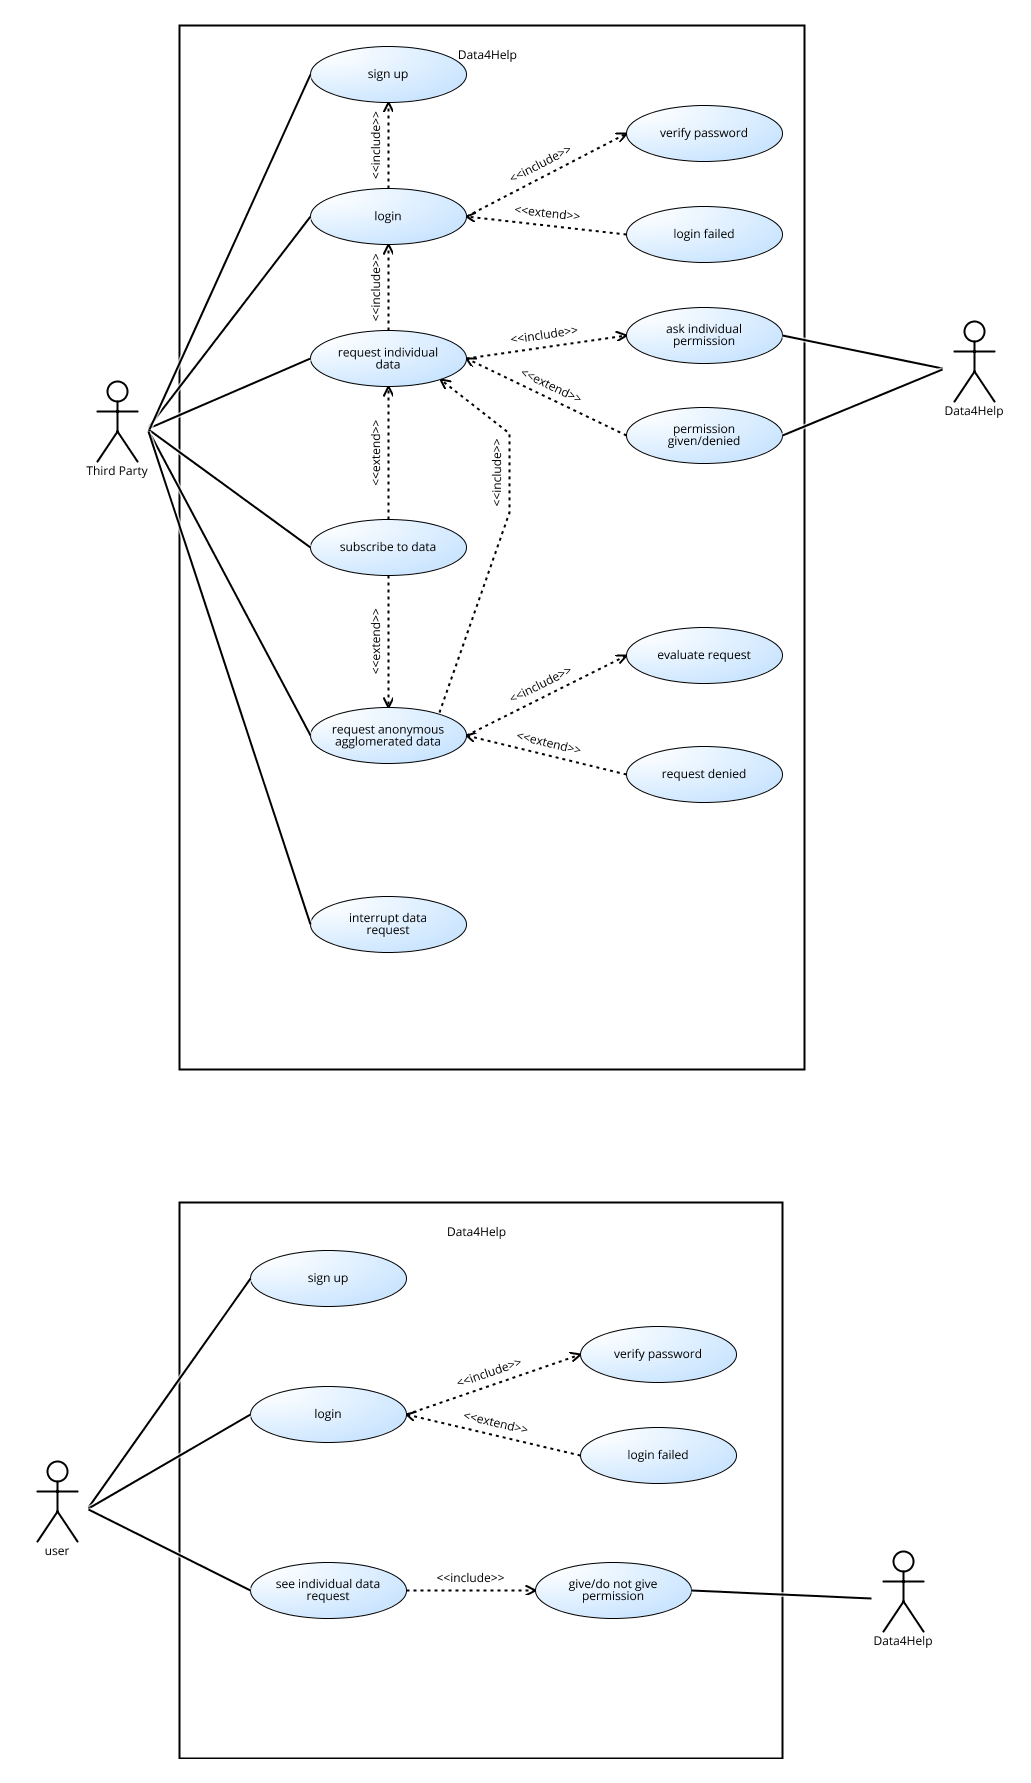
\includegraphics[width=\linewidth, height = 20cm, keepaspectratio]{./Images/RASD_Data4Help_Use_Case_Diagram.png}
    \centering
    \caption{Data4Help}
    \label{fig:sab}
  \end{figure}
\newpage
\begin{figure}[H]
    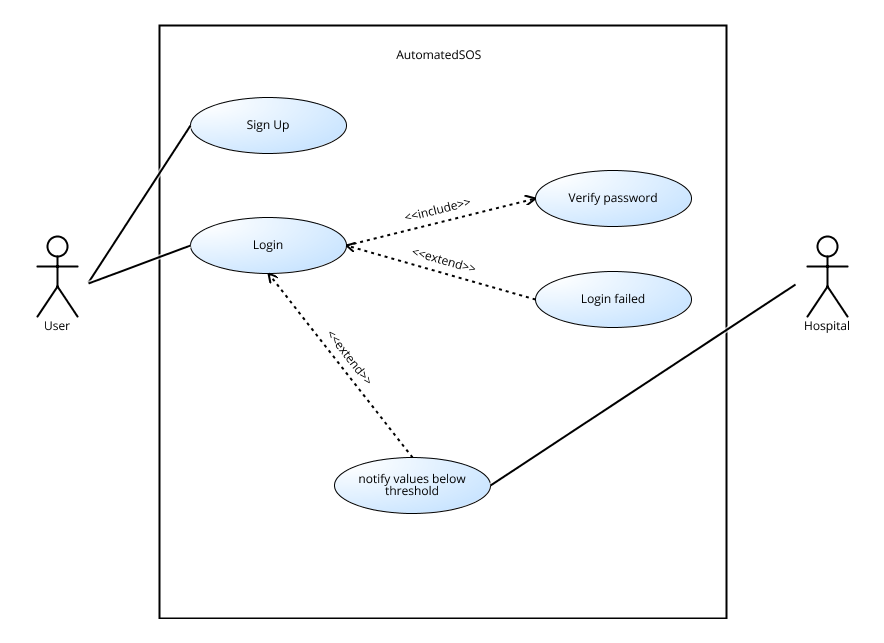
\includegraphics[width=\linewidth, height=10cm, keepaspectratio]{./Images/RASD_Automated_SOS_Use_Case_diagram.png}
    \centering
    \caption{AutomatedSOS}
    \label{fig:sab}
  \end{figure}
  
  
  \begin{figure}[H]
    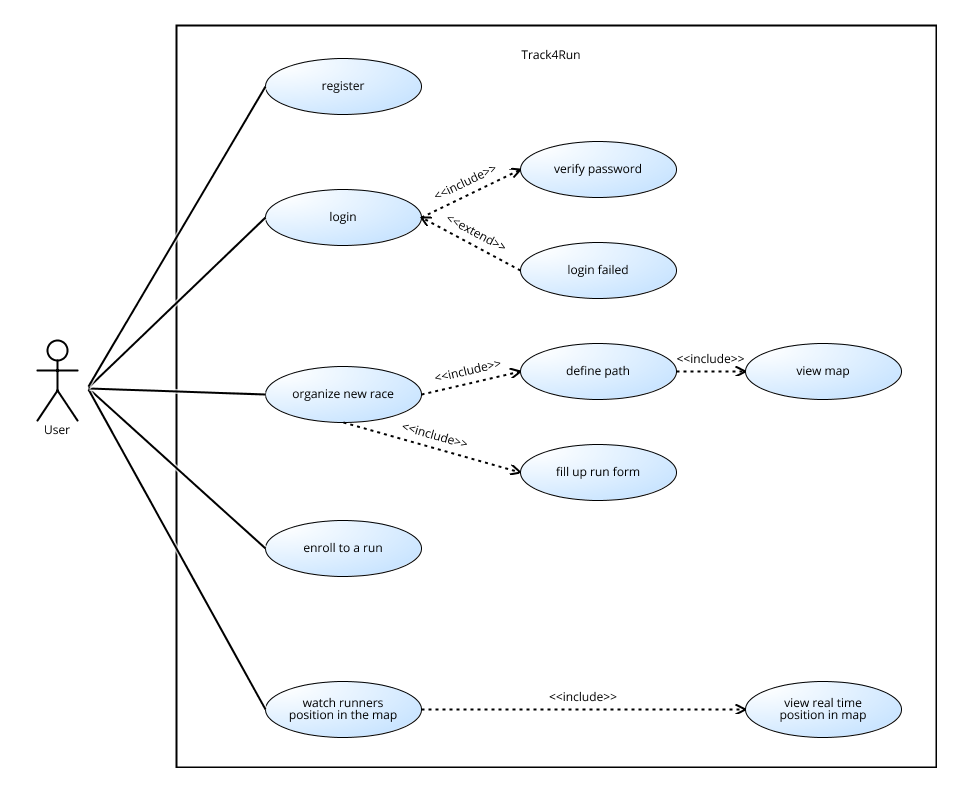
\includegraphics[width=\linewidth, height=10cm, keepaspectratio]{./Images/RASD_Track4Run_Use_Case_Diagram.png}
    \centering
    \caption{Track4Run}
    \label{fig:sab}
  \end{figure}


\begin{table}[]
\begin{tabular}{ll}
\hline
\multicolumn{1}{|l|}{Name}            & \multicolumn{1}{l|}{Sign up - Data4Help}    
 \\ \hline
\multicolumn{1}{|l|}{Actor}           & \multicolumn{1}{l|}{Third Party}                
 \\ \hline
\multicolumn{1}{|l|}{Entry condition} & \multicolumn{1}{l|}{the user has installed the application on his device}                                                                               
 \\ \hline
\multicolumn{1}{|l|}{Event flow}      & \multicolumn{1}{l|}{\begin{tabular}[c]{@{}l@{}}
1. Open the application and click on the "sign in" button\\ 
2. Fill up the form with his personal information, including his fiscal code\\ 
3. Agree with the privacy policy\\ 
4. Confirm the registration\\ 
5. The system saves the data in its database\end{tabular}}                                 
\\ \hline
\multicolumn{1}{|l|}{Exit condition}   & \multicolumn{1}{l|}{The user has successfully registered and is now able to use the service }                                                                                                                      
\\ \hline
\multicolumn{1}{|l|}{Exceptions}       & \multicolumn{1}{l|}{\begin{tabular}[c]{@{}l@{}}All the exceptions are handled by showing to the user a log which\\ explains the kind of exception. Moreover he is taken back to a refreshed\\ "sign up" page.\\ The possible exceptions are:\\ 
1. The email the user provided has already been used\\ 
2. The fiscal code the user provided has already been used \\     
(he has already registered)\\ 
3. The user does not fill all the mandatory info and clicks on "confirm"\\ 
4. The user does not agree with the privacy policy and clicks on "confirm"\end{tabular}}
\\ \hline
\end{tabular}
\end{table}



\begin{table}[]
\begin{tabular}{ll}
\hline
\multicolumn{1}{|l|}{Name}            & \multicolumn{1}{l|}{Login - Data4Help}                        \\ \hline
\multicolumn{1}{|l|}{Actor}           & \multicolumn{1}{l|}{Third Party}                              \\ \hline
\multicolumn{1}{|l|}{Entry condition} & \multicolumn{1}{l|}{the user has installed the application on his PC/Mac, registered and logged in}                                                                                               
\\ \hline
\multicolumn{1}{|l|}{Event flow}      & \multicolumn{1}{l|}{\begin{tabular}[c]{@{}l@{}}
1. Open the application and click on the "login" button\\ 
2. Insert VAT identification number\\ 
3. Insert password\\ 
4. Check VAT and password match\\ 
5. Enter the desktop application\end{tabular}} 
\\ \hline
\multicolumn{1}{|l|}{Exit condition}     & \multicolumn{1}{l|}{The user has successfully logged in and is now on the main page of the application}                                                      
\\ \hline
\multicolumn{1}{|l|}{Exception}          & \multicolumn{1}{l|}{\begin{tabular}[c]{@{}l@{}}All the exceptions are handled by showing to the user a log which\\ explains the kind of exception. Moreover he is taken back to a refreshed\\ "login" page.\\ The possible exceptions are:\\ 
1. The VAT identification number used is unknown by the system\\ 
2. The VAT identification number and the password do not match\\ 
3. The user does not fill the "VAT identification number" field and clicks on "confirm"\\ 
4. The user does not fill the "password" field and clicks on "confirm"\end{tabular}}
\\ \hline
\end{tabular}
\end{table}


\begin{table}[]
\begin{tabular}{ll}
\hline
\multicolumn{1}{|l|}{Name}            & \multicolumn{1}{l|}{Request individual data - Data4Help}     \\ \hline
\multicolumn{1}{|l|}{Actor}           & \multicolumn{1}{l|}{Third Party}                              \\ \hline
\multicolumn{1}{|l|}{Entry condition} & \multicolumn{1}{l|}{the user has installed the application on his PC/Mac, registered and logged in}
\\ \hline
\multicolumn{1}{|l|}{Event flow}      & \multicolumn{1}{l|}{\begin{tabular}[c]{@{}l@{}}
1. Click on the "new request" button from the homepage\\ 
2. Click on the "user's personal data" button \\
2. Fill form with the name of the individual, kind of data requested, \\     and a message to be shown to the individual\\ 
3. Click on the "send request" button\\ 
4. Receive response from the service\end{tabular}}                                      
\\ \hline
\multicolumn{1}{|l|}{Exit condition}     	& \multicolumn{1}{l|}{\begin{tabular}[c]{@{}l@{}}Two possibilities:\\ 
1. The TP receives the approval for the request and the asked data.\\ 
2. The TP receives a denial for the requested data\end{tabular}}                                     \\ \hline
\multicolumn{1}{|l|}{Exceptions}   		& \multicolumn{1}{l|}{\begin{tabular}[c]{@{}l@{}}All the exceptions are handled by showing to the actor a log which\\ explains the kind of exception. Moreover he is taken back to a refreshed\\ "request individual data" page.\\ The possible exceptions are:\\ 
1. The name inserted in the form does not match with any \\ name contained in the database\end{tabular}}
\\ \hline
\end{tabular}
\end{table}




\begin{table}[]
\begin{tabular}{ll}
\hline
\multicolumn{1}{|l|}{Name}            & \multicolumn{1}{l|}{Request anonymous aggregated data - Data4Help}                                                                                            \\ \hline
\multicolumn{1}{|l|}{Actor}           & \multicolumn{1}{l|}{Third Party}                              \\ \hline
\multicolumn{1}{|l|}{Entry condition} & \multicolumn{1}{l|}{the third party has installed the application on his PC/Mac, registered and logged in} 
\\ \hline
\multicolumn{1}{|l|}{Event flow}      & \multicolumn{1}{l|}{\begin{tabular}[c]{@{}l@{}}
1. Click on the "new request" button from the homepage\\ 
2. Click on the "anonymous aggregated data" button\\
3. Specify the kind of data requested (position, age, average heart beat rate,...)\\ 
4. Click on the "send" button\\ 
5. Receive response from the service\end{tabular}}  
\\ \hline
\multicolumn{1}{|l|}{Exit condition}    & \multicolumn{1}{l|}{\begin{tabular}[c]{@{}l@{}}Two possibilities:\\ 
1. The third party receives the approval for the request and the asked data.\\ 
2. The third party receives a denial for the requested data, because\\     the number of individual registered in such area that satisfies the criteria\\     chosen by the third party are less the 1000\end{tabular}}
\\ \hline
\multicolumn{1}{|l|}{Exceptions}         & \multicolumn{1}{l|}{\begin{tabular}[c]{@{}l@{}}All the exceptions are handled by showing to the user a log which\\ explains the kind of exception. Moreover he is taken back to a refreshed\\ "aggregated data request" page.\\ The possible exceptions are:\\ 
1. No data is requested from the third party and the "send" button is clicked\end{tabular}}
\\ \hline
\end{tabular}
\end{table}


\begin{table}[]
\begin{tabular}{ll}
\hline
\multicolumn{1}{|l|}{Name}            & \multicolumn{1}{l|}{Sign up - AutomatedSOS \& Track4Run}     \\ \hline
\multicolumn{1}{|l|}{Actor}           & \multicolumn{1}{l|}{User}                                     \\ \hline
\multicolumn{1}{|l|}{Entry condition} & \multicolumn{1}{l|}{the user has installed the app on his device}                                                                                               \\ \hline
\multicolumn{1}{|l|}{Event flow}      & \multicolumn{1}{l|}{\begin{tabular}[c]{@{}l@{}}
1. Click on the "sign up" button \\ 
2. Fill up the form with personal info \\ 
3. Click on the "confirm" button\end{tabular}}                                                        \\ \hline
\multicolumn{1}{|l|}{Exit condition}      & \multicolumn{1}{l|}{The user signs up and is ready to log in}
\\ \hline
\multicolumn{1}{|l|}{Exceptions}           & \multicolumn{1}{l|}{ \begin{tabular}[c]{@{}l@{}}All the exceptions are handled by showing to the user a log which\\ explains the kind of exception. Moreover he is taken back to a refreshed\\ "sign up" page.\\ The possible exceptions are:\\ 
1. The user does not fill all the mandatory information in the form and\\     clicks on the "confirm" button\\ 
2. The user does not agree with the privacy policy and clicks on the \\     confirm button\end{tabular}}
\\ \hline
\end{tabular}
\end{table}



\begin{table}[]
\begin{tabular}{ll}
\hline
\multicolumn{1}{|l|}{Name}            & \multicolumn{1}{l|}{Login - AutomatedSOS \& Track4RUn}        \\ \hline
\multicolumn{1}{|l|}{Actor}           & \multicolumn{1}{l|}{User}                                     \\ \hline
\multicolumn{1}{|l|}{Entry condition} & \multicolumn{1}{l|}{the user has installed the app on his device and signed up}                                                                                 \\ \hline
\multicolumn{1}{|l|}{Event flow}      & \multicolumn{1}{l|}{\begin{tabular}[c]{@{}l@{}}
1. Click on the "login" button \\ 
2. Insert email\\ 
3. Insert password\\ 
4. Click on the "confirm" button\end{tabular}}                                                        \\ \hline
\multicolumn{1}{|l|}{Exit condition}    & \multicolumn{1}{l|}{The user logs in  and is ready to use the service}
\\ \hline
\multicolumn{1}{|l|}{Exceptions}         & \multicolumn{1}{l|}{\begin{tabular}[c]{@{}l@{}}All the exceptions are handled by showing to the user a log which\\ explains the kind of exception. Moreover he is taken back to a refreshed\\ "login" page.\\ The possible exceptions are:\\ 
1. The user inserts an e-mail address unknown by the system's database\\ 
2. The user inserts a known e-mail address but the password he inserts \\     does not match the provided e-mail\end{tabular}}
\\ \hline
\end{tabular}
\end{table}


\begin{table}[]
\begin{tabular}{ll}
\hline
\multicolumn{1}{|l|}{Name}            & \multicolumn{1}{l|}{Organize new run - Track4Run}             \\ \hline
\multicolumn{1}{|l|}{Actor}           & \multicolumn{1}{l|}{User}                                     \\ \hline
\multicolumn{1}{|l|}{Entry condition} & \multicolumn{1}{l|}{the user has installed and logged in the application on his device}                                                                            \\ \hline
\multicolumn{1}{|l|}{Event flow}      & \multicolumn{1}{l|}{\begin{tabular}[c]{@{}l@{}}1. Click on the "organize" button\\ 2. Fill up form with name of the event, date, location\\ 3. Click on the "confirm" button\\ 4. Select path from available paths by:\\ 4a. choosing start point from available street\\ 4b. choosing end point from such street\\ 5. Choose between going back to 4a. or ending path\\ 6. Click on the "confirm" button\end{tabular}}                                                     \\ \hline
\multicolumn{1}{|l|}{Exit condition}     & \multicolumn{1}{l|}{The user has successfully organized the run}
\\ \hline
\multicolumn{1}{|l|}{Exception}       & \multicolumn{1}{l|}{\begin{tabular}[c]{@{}l@{}}All the exceptions are handled by showing to the user a log\\ which explains the kind of exception. Moreover he is taken back\\ to a new "Organize new run" page.\\ The possible exceptions are:\\ 1. The user forgets to fill at least one of the field in the form and\\     clicks on the "confirm" button.\\ 2. The city selected to organize the run in is not recognized\\      by the Track4Run systems, which means that Track4Run\\     does not own a stylized map of such city.\end{tabular}}
\\ \hline
\end{tabular}
\end{table}

\newpage

{\color{secblue}\subsubsection{Sequence diagrams}}

\begin{figure}[H]
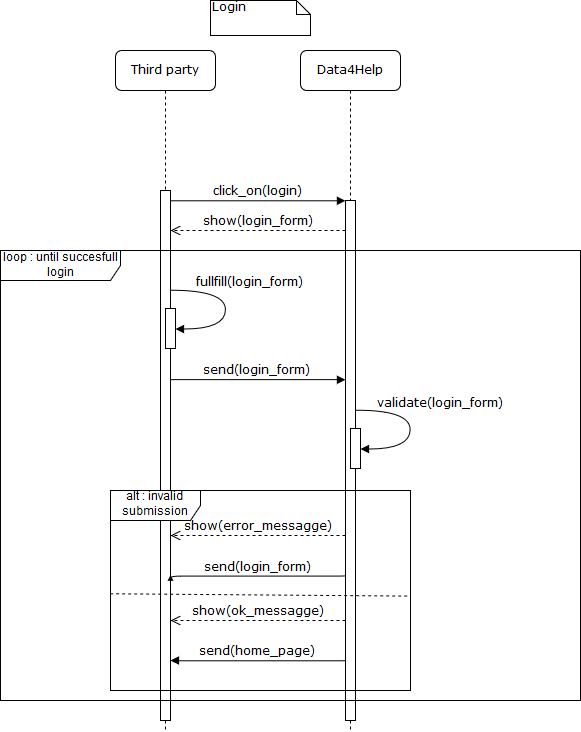
\includegraphics[width=\linewidth, height=9cm, keepaspectratio]{./Images/sequence_diag_login.png}
\centering
\caption{Login sequence diagram}
\end{figure}

\begin{figure}[H]
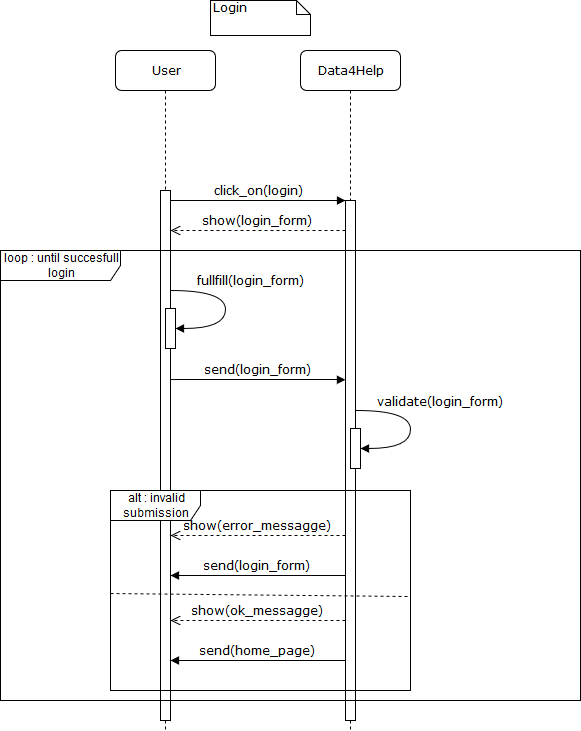
\includegraphics[width=\linewidth, height=9cm, keepaspectratio]{./Images/sequence_diag_login_user.png}
\centering
\caption{User's login sequence diagram}
\end{figure}

\begin{figure}[H]
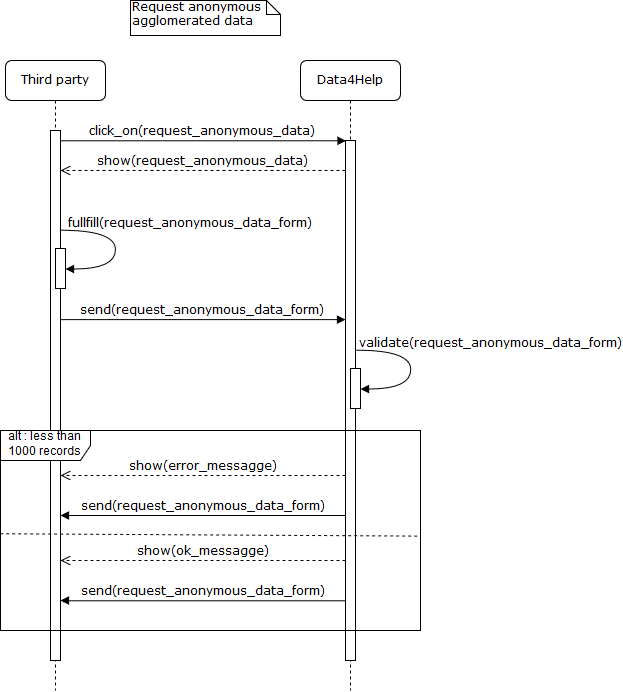
\includegraphics[width=\linewidth, height=9cm, keepaspectratio]{./Images/sequence_diag_request_anonymous_agglomerated_data.png}
\centering
\caption{Request anonymous agglomerated data sequence diagram}
\end{figure}

\begin{figure}[H]
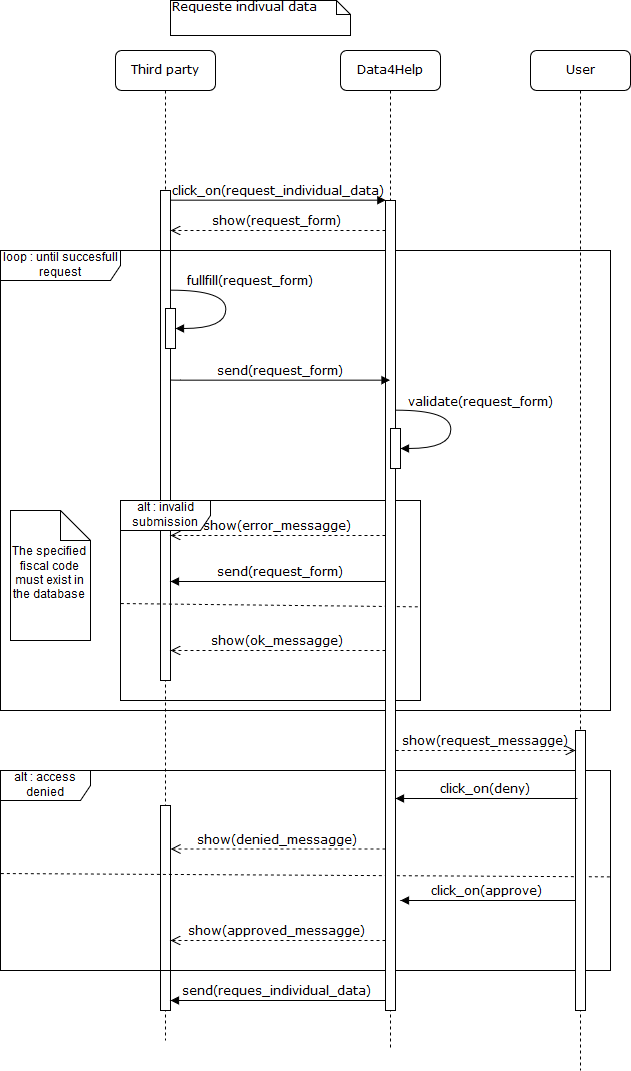
\includegraphics[width=\linewidth, height=11cm, keepaspectratio]{./Images/sequence_diag_request_individual_data.png}
\centering
\caption{Request individual data sequence diagram}
\end{figure}

\begin{figure}[H]
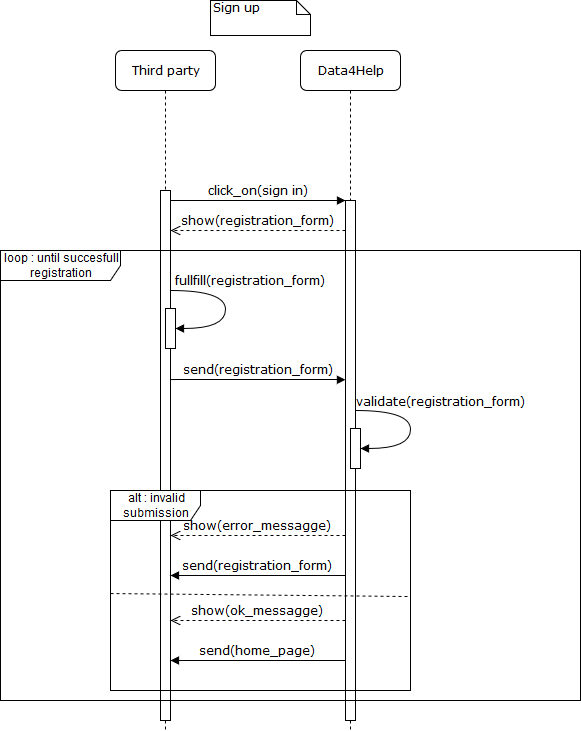
\includegraphics[width=\linewidth, height=10cm, keepaspectratio]{./Images/sequence_diag_sign_up.png}
\centering
\caption{Sign up sequence diagram}
\end{figure}

\begin{figure}[H]
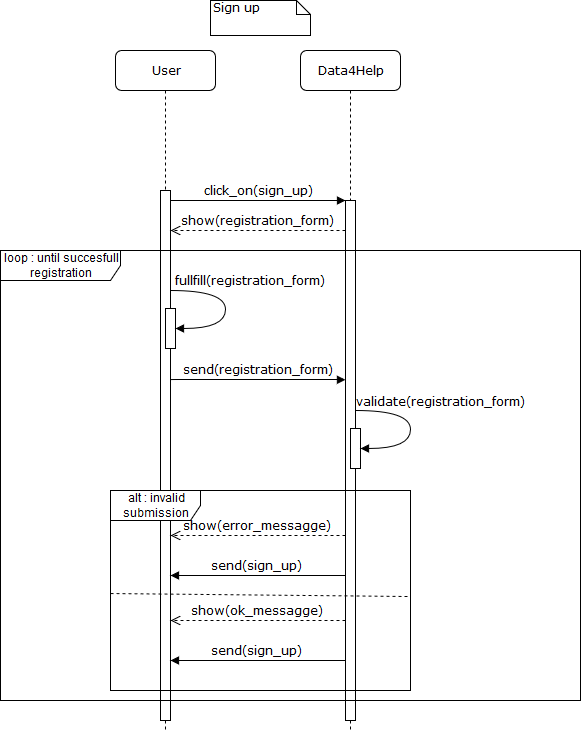
\includegraphics[width=\linewidth, height=10cm, keepaspectratio]{./Images/sequence_diag_sign_up_user.png}
\centering
\caption{Sign up user sequence diagram}
\end{figure}

\begin{figure}[H]
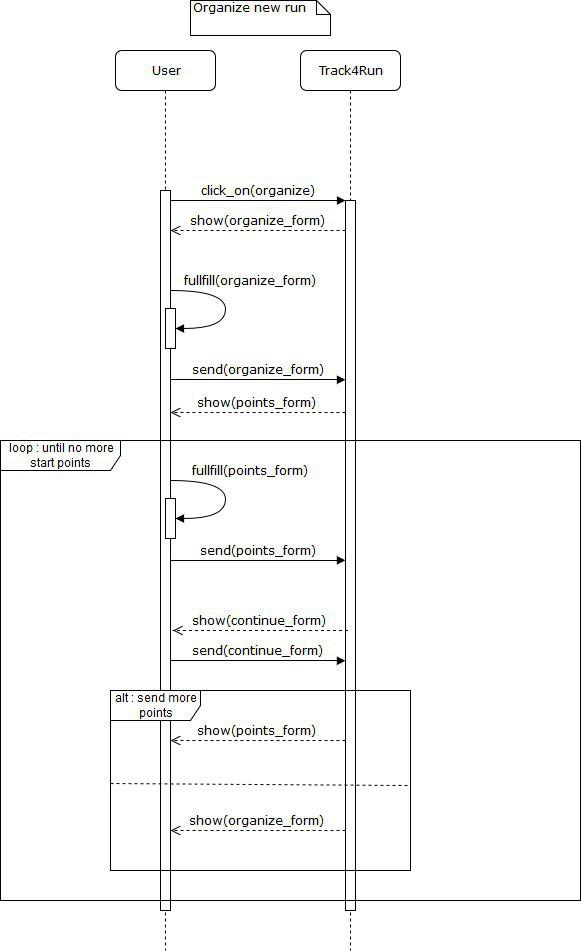
\includegraphics[width=\linewidth, height=10cm, keepaspectratio]{./Images/sequence_diag_new_run.jpg}
\centering
\caption{New run sequence diagram}
\end{figure}
\newpage
{\color{secblue}\subsubsection{Mapping on requirements}}
\begin{itemize}
\item [G1] - The Data4Help application gives constantly new data accordingly to users' activities.
This is achieved with [D1], [D2], [R8], [R9], [R10], [R11], [R13], [R14],\\
\textbf{[FR1]} - The users must be logged in
\item [G2] - Registered TPs (Third Parties) can send request to specific users if they know their SSN or CF to retrieve their specific data.
This is achieved with [R2], [R3], [R8], [R10], [FR1], \\
\textbf{[FR2]} - the users have the possibility of accepting or refusing a non-anonymous data requests. \newline
\textbf{[FR3]} - The TP must be logged in.


\item [G3] - Registered TPs have access to make queries to Data4Help's database to get specific data by filtering by one or more parameters as they need.
This is achieved with [D2], [R1], [R2], [R3], [R7], [R8], [R10], [R11], [FR3]


\item [G4] - Results for TPs' queries are given only if the number of matches is greater or equal than 1000.
This is achieved with [R1], [R2], [R7].


\item [G5] - Each user of the services offered by TrackMe is identifiable in order to gather his data and to communicate with him.
This is achieved with 
[R6], [FR1], [R12], \\
\textbf{[FR4]} - the users must register in the system in order to be identified.

\item [G6] AutomatedSOS sends automatically a request when and only when some user's values are below a specific critical threshold, specifying the user's position.
This is achieved with [D1], [D2], [D3], [D4], [R5], [R6], [R9], [R10], [R11], [R14], [FR1], \\
\textbf{[FR5]} - The hospitals need to be always available in case of emergency call, this means that there is always an ambulance and some personnel available. \\
\textbf{[FR6]} - The users of AutomatedSOS need to have their sensors equipped devices connected to the system in order to be helped.


\item [G7] - Users of Track4Run are able to create a run defining the precise path.
This is achieved with [R1], [R6], [R7], [R14], [FR1], \\
\textbf{[FR7]} - The users of Track4Run, whenever they want to organize a new run, need to insert reasonable gps coordinates in the definition of the path. \\
\textbf{[FR8]} - The users of Track4Run, whenever they want to organize a new run, need to have the permission of the city hall in case the path defined is public land.
\item [G8] - Users of Track4Run are able to take part in a created run as runners.
This is achieved with [R7], [R14], [FR1], \\
\textbf{[FR9]} - The users of Track4Run, whenever they take part in a run, need to wear their gps equipped device in order to be tracked.
\item [G9] - Users of Track4Run can see real-time runners' positions of runs in which they are subscribed.
This is achieved with [D5], [R4], [R7], [R11].
\end{itemize}

{\color{secblue}\subsection{Performance requirements}}
[R7] - Performance plays a big role in all the 3 projects: regarding the Data4Help and Track4Run they both have to manage a large amount of people that can range from 0 (i.e.: an event organized through Track4Run) to 10000 (i.e.: a fair amount of user that we should excpect from Data4Help) based on the current users requests. Regarding the AutomatedSOS there isn't a specific need for performance, but for reliability, which is explained in the reliability section.
{\color{secblue}\subsection{Design constraints}}
{\color{secblue}\subsubsection{Standard compliance}}
[R8] - Internally the data that is collected through Data4Help can be stored in any way that is comfortable for the developers to work with, but when it is delivered to the third parties it must use a standard format.
This means that:
\begin{enumerate}
\item - R8.1 - the TP can choose of receiving the results of its requests in the form of a summary in a PDF file.
\item - R8.2 - the TP can choose of receiving the results of its request in a database file, in such a way that the third parties can manipulate the data the way they like.
\item - R8.3 - The TP can request both the formats above.
\end{enumerate}
{\color{secblue}\subsubsection{Hardware limitations}}
The services to be developed would work on any of the smartphones available in the market because the technologies needed for such services in order to work are very basic (bluetooth connection with the sensors equipped devices, gps and internet connection).

{\color{secblue}\subsubsection{Any other constraints}}
[R9] - Bandwidth may be a constraint, because developers need to pay attention to send only the essential data from the sensors equipped device to the server, because in an hypotetical situation the application may drain too much mobile data from the users' sensors equipped device. To achieve this is possible also to set a reasonable amount of time to be waited between each single user's update of his/her values to the server. On the contrary, AutomatedSOS doesn't have any bandwidth limitation.
{\color{secblue}\subsection{Software system attributes}}
{\color{secblue}\subsubsection{Reliability}}
[R10] - Reliability is the main concern for AutomatedSOS, because of the nature of the service itself, and surely is important in the development of the Data4Help module. Secondly, reliability is not the main concern in Track4Run.
The whole system should at least be 99.999\% reliable.
{\color{secblue}\subsubsection{Availability}}
[R11] - AutomatedSOS needs a six 9s (99.9999\%) availability, due to the high importance availability plays for this service, while Data4Help and AutomatedSOS need at least a five 9s (99.999\%) availability.
{\color{secblue}\subsubsection{Security}}
[R12] - Anonymization must be granted giving the fact that we are working with very sensible data.
Since AutomatedSOS and Track4Run talk with Data4Help, this means that the communication between the modules must be protected as well. 

{\color{secblue}\subsubsection{Mantainability}}
[R13] - Mantainability is a big concern for all the three services. Given the fact that the application is mainly developed for Android and iOS, it must be easily maintainable, because of the frequent updates of both the operating systems. This translates in the decoupling of the components of the system.

{\color{secblue}\subsubsection{Portability}}
[R14] - The application that is developed for Data4Help users must work for all iOS' and Android's updates by the date of launch of the app. The same can be applied to Track4Run and Automated SOS because it's not easy to foresee how smartwatches' and smartphones' market will change in the future. The desktop application of Data4Help instead has not the same portability requirements, because, being developed for the Windows operating system, we can rely on his well established legacy of portability.
{\color{secblue}\subsection{Scenarios}}
{\color{secblue}\subsubsection{Scenario 1 - Data4Help}}
Data Request:
A local newspaper of the city of Padova wants to write an article about the average 
age of the people visiting the city so one of the journalists opens the Data4Help account of his journal on his PC.
He finds himself in the homepage of the application and clicks on the "New Request" button. Then He clicks on the "anonymous aggregated data" button.
Afterwards a few text fields pop up and he fills them with requesting to the system the age of the people that in the last month
spent at most one week in the city. Done so, he asks for a monthly update. He clicks on "send" and waits for the approval of the request.
After a few seconds the system approves the request and provides him with a list of numbers corresponding to the ages of such people (such list is provided monthly as requested).


{\color{secblue}\subsubsection{Scenario 2 - Data4Help}}
Data Request Denied:
The touristic office of Santa Lucia, a small town in Sardegna wants to understand how many non italian tourists come visit the city in the summer, so they request data for all the foreigners spending at most 2 weeks in the city (doing the same procedure explained in the scenario above), asking for a 2 weeks update.
After 2 weeks Data4Help tells the touristic office, through the in-app notification software, that they can't release the information collected because the number of people who visited the town in that period are less than 1000.
In such message Data4Helps tells to the office that they can ask to collect data for the coming next two weeks. 

{\color{secblue}\subsubsection{Scenario 3 - Data4Help}}
Request Interruption:
A company that sells school items is willing to open a new shop in Milan. 
They want to maximize the number of customers visiting their shop so they ask to Data4Help to provide them with the data of the people living in Milan who are between 6 and 20 years old. 
The service provides to the company the position of each of such individuals, updated hourly.
After six months the company is satisfied with the data they have collected, and understands that the part of the city where there is the highest flux of students is Città Studi.
So the CMO of the company goes to the homepage of the Data4Help app, clicks on the query he wants to interrupt, and then clicks on the query interruption button. 
The app responds with a log stating that the removal of the request was successful.

{\color{secblue}\subsubsection{Scenario 4 - Data4Help}}
Company registration and login:
A sportwear company called RunUp wants to start a series of running events in Rome in order to
promote their products and their philosophy.
The company asks to the chief marketing officer to organize the calendar of events 
that will be held in Rome.
So he downloads the desktop application on his PC and he opens it.
The application recognizes this is the first time that it's being opened, so a signing up page gets opened.
He registers his company and a form pops up.
Such form has 4 fields: company's name, email, VAT number and password.
He fills such fields and clicks on the "confirm" button.
The Data4Help Staff activates the company's account and the CMO is ready to log in, so he opens the application, clicks on the "Log in" button from the homepage and inserts the VAT number and password in the relative fields.
He clicks on the "confirm" button and he's redirected to the his personal space's page.
Now the CMO can use the application to make his request to the system.

{\color{secblue}\subsubsection{Scenario 5 - Data4Help}}
User's Sign up and Login:
John is a 25 years old man who wants to enroll in the gym nearby his house.
He enters the gym and fills up the enrollment form.
At the bottom of such form he is asked through a check box whether he wants to register in Data4Help. Doing so his phone could provide data to the gym, that would be used to help the trainers assigning targeted exercises to John.
He checks the box and gives the filled form to the gym's secretary. 
Then he takes his iPhone, downloads the app from the Apple Store, opens it and the "sign up" page of the app appears on the screen.
Such form consists in seven fields: name, lastname, nationality, age, SSN (or fiscal code), email, and password.
He fills all of such fields, checks the privacy policy box,  and clicks on the "Confirm" button, so joining the users' community of Data4Help.
He gets redirected to the "login" page which consists of two fields: email and password.
He fills such fields and clicks on the "confirm" button, being redirected to the home of the app, where he can see the devices paired with his phone and a table containing all the data provided by the sensors paired with his phone.

{\color{secblue}\subsubsection{Scenario 6 - AutomatedSOS}}
User's Sign up, Log in \& Pairing:
Maria is a 80 years old woman, which sometimes happens to have difficulties in breathing. 
This is why she bought a smart blood-oxygen levels sensor that she constantly wears.
Since her doctor notices she bought such device, he suggests her to download the AutomatedSOS app.
She goes to the Play Store with her Android smartphone and downloads it. 
Once she downloads it she opens it and the app shows the "sign up" page. Such page consists in a form with seven fields:
name, last name, nationality, age, SSN (or Fiscal Code), email and password.
She fills such fields, checks the privacy policy box and clicks on the "confirm" button.
She gets redirected  to the Log in page, where she fills the email and password fields and clicks on the "confirm" button.
Now she gets to the homepage of AutomatedSOS, from where she can pair her sensor via bluetooth to the app. 
She manage to do it by clicking on the "Plus" icon, the smartphone finds the sensor and Maria agrees on pairing the devices.

{\color{secblue}\subsubsection{Scenario 7 - AutomatedSOS}}
Help request:
Walter is a 70 years old man which suffers from asthma, this is why he installed AutomatedSOS on his smartwatch.
One evening he is at a friend's house and he has an asthma attack but he forgot his inhaler at home.
His smartwatch notices an above-average hearth rate and AutomatedSOS calls an ambulance for him, to be sent at the location of his friend's house.
The ambulance arrives in time, knowing he suffers from asthma, the nurses brought along an inhaler to be given to him.
He uses the inhaler and his breath goes back to normal.

{\color{secblue}\subsubsection{Scenario 8 - Track4Run}}
Partecipant signs up and logs in:
Anna is an university student who studies in Zurich.
One monday morning, after class, she notices that her university, the University of Zurich, is organizing a half-marathon by the lake of Zurich.
On the bottom of the flyer is written that in order to partecipate, each runner has to register via Track4Run.
Since she owns an Android smartphone, she downloads the app from the Play Store, and opens it.
The "Sign up" page gets displayed. 
Such page consists in a form to be filled containing the following fields:
name, last name, nationality, age, SSN / fiscal code, email, and password. 
She fills such fields, checks the privacy policy box and clicks on the "confirm" button.
Right after she is told her account has been activated and opens the log in page.  
She fills the email and password fields and clicks on the "confirm" button.
Now she can succesfully enroll in the run organized by her university.


{\color{secblue}\subsubsection{Scenario 9 - Track4Run}}
Organizing run \& registration:
Mike is a loyal user of Track4Run.
One day he decides to organize a run in the main park of his town, Windsor. 
He opens the Track4Run app on his smartphone and logs in.
He gets redirected to the homepage of the app, where he can decide whether he wants to organize, take part or watch a run.
He clicks on the "Organize" button and a new page opens where he needs to fill up a form inserting the name of the run, the date and time (up to minute precision), and the city where such run will be held.
He clicks on the "confirm" button and a map gets displayed from which he can select among many available paths or combinations of such paths.
The selection happens by simply clicking on one of the many streets displayed by the map, selecting a starting point and an ending point (such ending point must correspond to a crossroad or to the actual arrival point of the run).
Such process will be repeated until an arrival point will be defined.
Once the path is defined Mike clicks on the "end here" button and waits for the approval of Track4Run.
Het gets told that the partecipant can take part to such new run.
The day of the competitions arrives, and the event reveals to be a success, due to the high amount of people taking part in it.

{\color{secblue}\subsubsection{Scenario 10 - Track4Run}}
Watch run:
Gabriel is a 50 years old man who has a 15 years old son, Mike.
Mike is going to take part to a 10 km local run held in his hometown, Pavia, this sunday, which has been organized via Track4Run.
Gabriel is a big fan of his son, unfortunately he will be abroad for work during the weekend, but he knows that he can log in Track4Run as a spectator during the run of his son.
On sunday he opens the app and the homepage of the app gets displayed. Here he can choose to click one out of three buttons:"organize", "take part" or "watch".
He clicks on the third one and a text field gets displayed. In such field he will write the city the run will be held in, namely Pavia.
After doing so he clicks on the "confirm" button.
Now a list with the run held in Pavia gets shown, he clicks on "Local Run" out of the list and on the "confirm" button.
Now a map displaying a progress bar, and a map of the path gets shown (the runners are represented by a circle inside which there is their id). 
Now Gabriel can watch his son's peformance from his hotel apartment.

{\color{secblue}\subsubsection{Scenario 11 - Track4Run}}
Taking part in a Run:
David is a professional runner.
One day, while surfing the internet, he notices that a run will be held in his city, London, in a week.
In order to register to the run he will need to enroll via Track4Run. Being a professional runner he already downloaded, signed up and logged in the app.
He now just needs to click on the "take part" button in the homepage of the app. 
A text field gets shown to him, in which he writes the name of the city where such run will be held, namely London. 
Afterwards he clicks on the "confirm" button. 
Now a list of run held in London is shown to him, from which he selects "London's half-marathon 2018" and clicks on the "confirm" button.
Right after he receives an email with all the run's information.

